%\addcontentsline{toc}{section}{\textbf{Annexe}}

\chapter{Inversion à partir d'une acquisition réaliste \label{annexe:acqui}}
Un exemple d'inversion monoparamètre de la vitesse est présenté ici, à partir d'une acquisition qui n'est pas en contact avec le relief de la soudure. Deux barrettes de 64 éléments espacées de 1 mm sont placées de chaque côté de la racine de la soudure. Les données sont générée à partir d'une soudure de masse volumique uniforme d'une valeur de 8000 kg/m$^{3}$ et de vitesse présentée en figure~\ref{app:iso:reel1}. La durée des signaux acquis est de 30.7 $\mu s$, ce qui est le temps nécessaire à la propagation d'une extrémité à l'autre du système d'acquisition. Le modèle initial de vitesse est uniforme, avec $v_{p}=6000$~m/s. Le modèle pour la masse volumique est fixé à sa valeur vraie.\\

 Le résultat de l'inversion, réalisée sur des fréquences allant de 200 k à 5 MHz, est présenté en figure~\ref{app:iso:reel2}. Il illustre à nouveau la dépendance de la résolution vis à vis du système d'acquisition. En effet, la racine de la soudure est mal reconstruite dans cette zone car les diffractions mesurées sont d'angle nul ou proche de $\pi$. Or, les angles de diffraction proches de $\pi$  contribuent à une reconstruction de résolution très faible, d'après l'expression du nombre d'onde~\ref{app:nb_onde}. Pour une application de la FWI à un cas réel, il est donc nécessaire de déterminer au préalable l'acquisition favorisant un éclairage adapté à la géométrie de la pièce à évaluer.
 
\begin{figure}[!h]
	\begin{subfigure}[b]{0.5\textwidth}
		\centering
		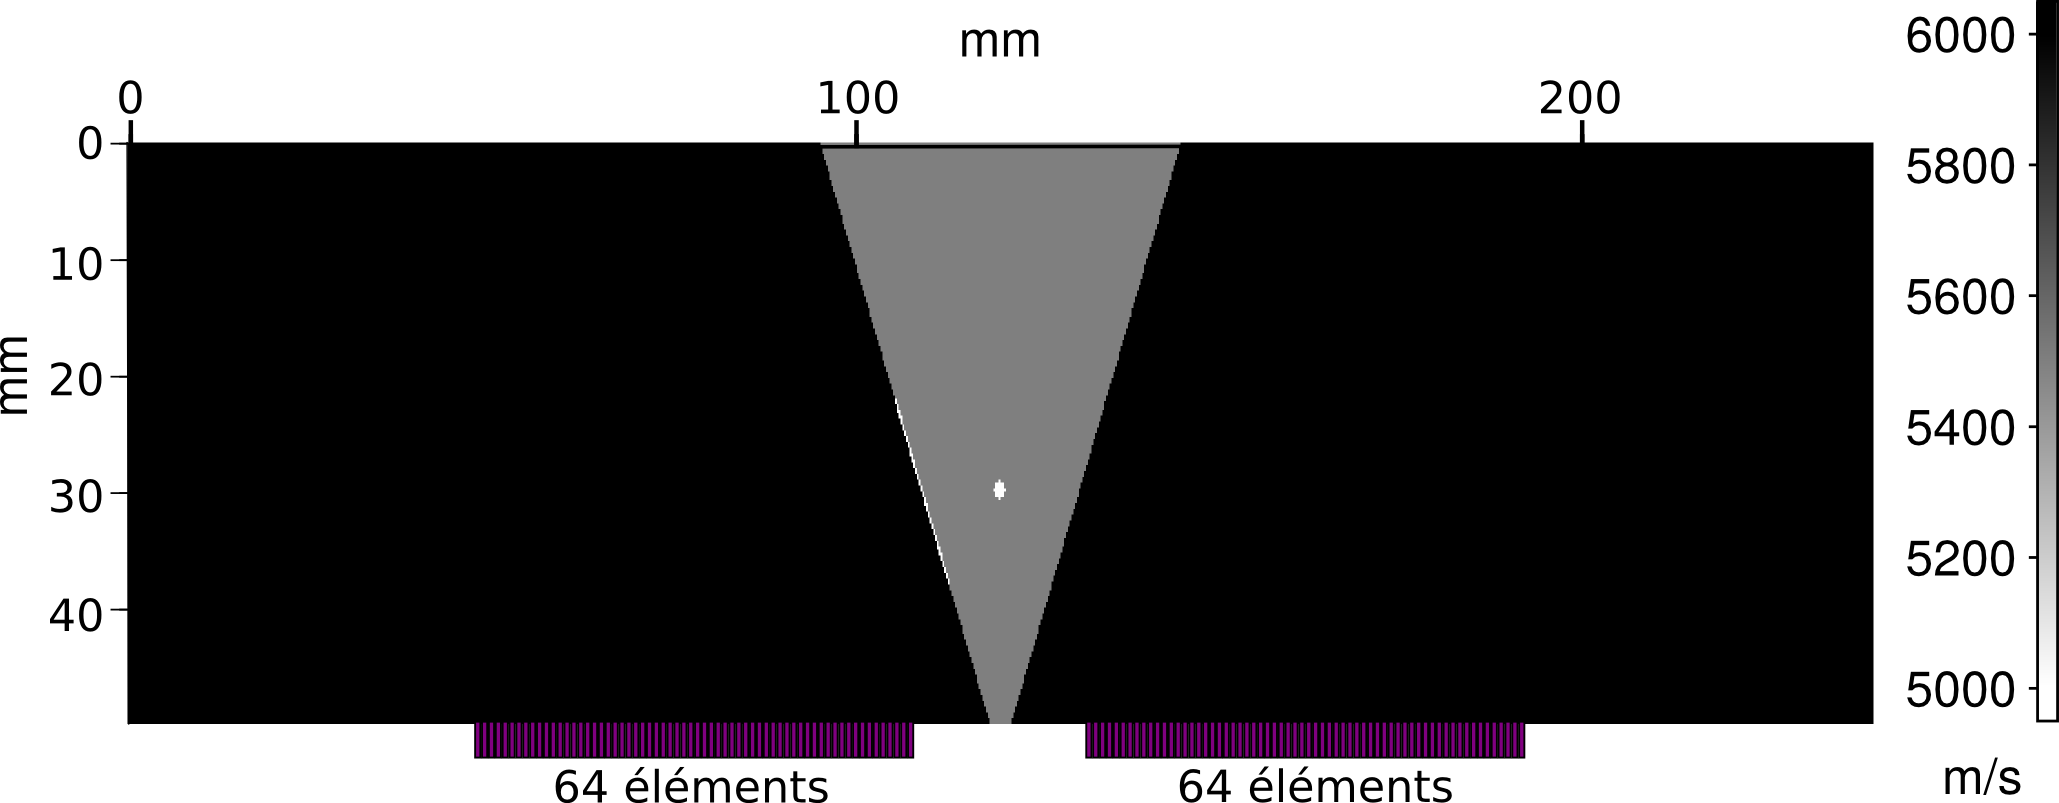
\includegraphics[width=\textwidth]{img/config_reelle_true.png}
		\caption{Configuration du système d'acquisition et vitesse utilisée pour la génération des données.\label{app:iso:reel1}}	
	\end{subfigure}
	\hspace{0.2cm}
	\begin{subfigure}[b]{0.5\textwidth}
		\centering
		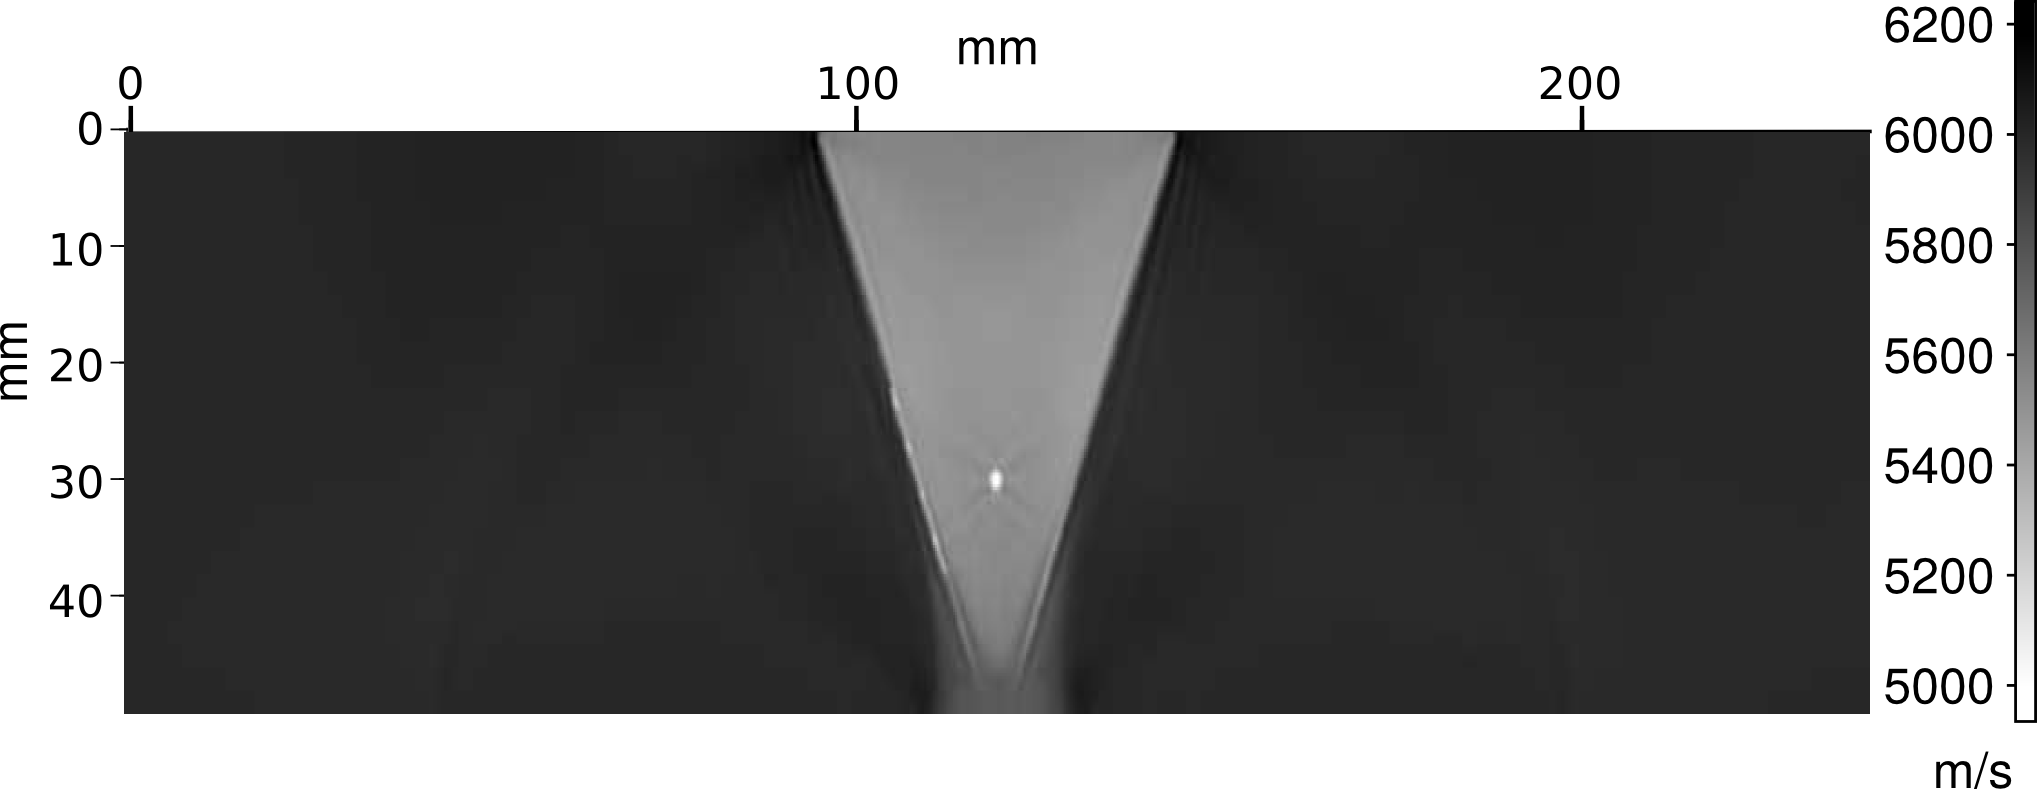
\includegraphics[width=\textwidth]{img/config_reelle_rec.png}
		\caption{Vitesse reconstruite par inversion monoparamètre. \label{app:iso:reel2}}	
	\end{subfigure}
	\caption{Exemple d'inversion pour une acquisition unilatérale. Chaque barrette est utilisée en excitation et en réception.}
\end{figure}



\chapter{Discrétisations et ressources nécessaires à l'inversion \label{annexe:chiffres}}

\section*{Discrétisation spatiale}
La résolution du problème direct par différences finies d'ordre 4 en espace sur maillage décalé nécessite de prendre un pas de discrétisation spatiale d'au moins 5 points par longueur d'onde \citep{levander}, afin de limiter la dispersion numérique.\\

Considérant que la plus petite longueur d'onde propagée est à 4 MHz, pour une vitesse minimale des ondes de compression de 5000 m/s, le pas de discrétisation spatiale choisi pour la propagation des ondes en milieu acoustique est $\Delta x=0,25$~mm.

\section*{Discrétisation temporelle}

Considérant un schéma à l'ordre 2 en temps et un espace à 2 dimensions, \cite{levander} préconise de respecter le critère de stabilité  
\begin{equation}
	\Delta t \leq \frac{\Delta x}{(c_{1}+c_{2})\sqrt{2} c_{max}},
\end{equation}
avec $c_{1}=\nicefrac{1}{24}$ et $c_{2}=\nicefrac{9}{8}$. En considérant une vitesse maximale de 6500 m/s et avec le pas de discrétisation spatiale choisi précédemment, il faut donc que 

\begin{equation}
	\Delta t \leq 2,3.10^{-8} \text{~s.}
\end{equation}
Respectant cette condition, la discrétisation spatiale utilisée pour tous les calculs de problème direct de cette étude est $\Delta t=1,5.10^{-8}$~s.



\section*{Ressources numériques}

Les inversions présentées dans ce rapport sont le résultats d'une suite d'inversions réalisées successivement à partir des données de références filtrées dans 9 gammes de fréquences, allant de 100 k à 3,4 MHz. 9 inversions sont donc réalisées, comportant chacune 20 perturbations successives du modèle.\\

Les calculs ont été réalisé sur les machines du centre de calcul CIMENT \footnote{Calcul Intensif / Modélisation / Expérimentation Numérique et Technologique : https://ciment.ujf-grenoble.fr}. Le temps de calcul nécessaire à une inversion (pour une seule gamme de fréquence) à 128 sources, est d'environ 5 minutes sur 128 cœurs  (sur des nœuds constitués de 8 biprocesseurs\footnote{d'architecture Sandy Bridge, Intel}, soit 16 cœurs par nœud).\\

 À titre de comparaison,  le calcul TFM prend une dizaine de minutes sur un ordinateur personnel\footnote{2 coeurs, 4 threads (processeur i7-4600u, Intel)} (pour une discrétisation spatiale semblable à celle utilisée pour la FWI).



%\section{Note sur les dimensions des grandeurs du chapitre \ref{fwi}}
%
%Les matrice $A$, qui est l'opérateur de l'équation d'onde a les dimensions de l'espace du problème direct : $l\times l$, où $l=n_{x}\times n_{z}$, $n_{x}$ et $n_{z}$ étant les dimensions du milieu de propagation discrétisé.\\
% De la même façon, le champ d'onde $\bm{u}$ et le vecteur source $\bm{s}$ sont de dimension $l\times 1$.\\
%Or, les vecteurs de données $\bm{d}$ ne contiennent que les informations aux $n$ points de réception. Ils sont donc de dimension $1\times n$. Les calculs sont donc menés sur des vecteurs agrandis à l'aide de zéros de façon à ce que $\bm{d}$ soit de dimension $l\times 1$. \\
%Finalement, le gradient  $\frac{\dd C (\bm{m})}{\dd \bm{m}}$ est bien de dimension $M\times 1$ avec $M$ le nombre de paramètre du problème \citep{pratt_98}.